%%=============================================================================
%% Methodologie
%%=============================================================================

\lstset{
	basicstyle=\ttfamily,
	columns=fullflexible,
	frame=single,
	breaklines=true
}

\chapter{\IfLanguageName{dutch}{Proof of Concept}{Proof of Concept}}
\label{ch:proofofconcept}

\section{Setting up a new Drupal 9 site}

Creating a new Drupal 9 site with the standard Drupal 9 profile on a local server environment is fairly simple. Some different steps are involved depending on the Operating System, but overall the workflow goes like this: 
\begin{itemize}
	\item Create a local environment using an AMP (Apache HTTP server, MySQL relational database, PHP programming language) stack. On the most popular OSs, Linux, Windows and MacOS, packages are available that include all of these technologies. These allow for a smooth and simple process of installing a local environment.
	\item Installing Drupal. The latest release of Drupal can always be found on the \url{https://drupal.org} site.
\end{itemize}

\subsection{Setting up a local environment}

In this proof of concept, MAMP will be used to create a local server environment. MAMP is a tool for MacOS that allows you to easily set up such an environment. The folder structure provided by MAMP should look like in figure \ref{fig:MAMP_Structure}. The most important directory here will be the htdocs directory. This folder will house all the Drupal files. 

\begin{figure}
	\centering
	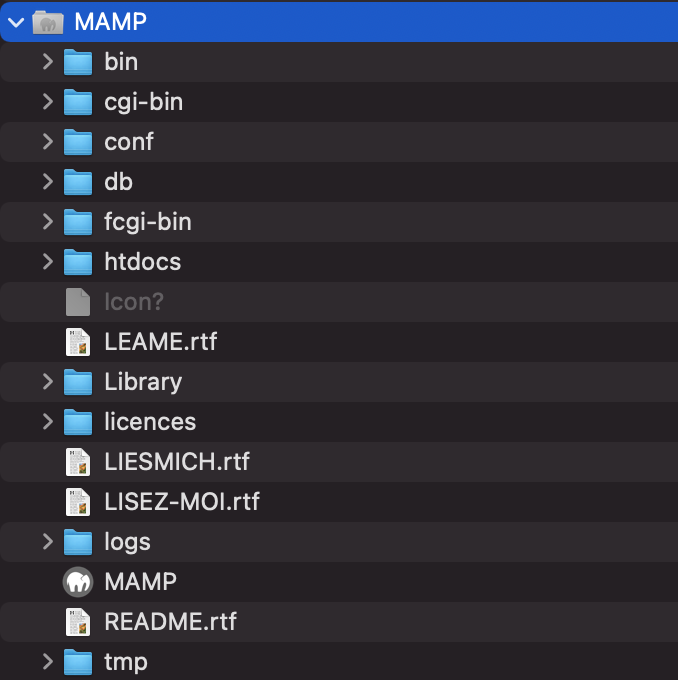
\includegraphics[width=10cm]{./img/MAMP_Structure.png}
	\caption[MAMP folder structure]{The folder structure provided by MAMP}
	\label{fig:MAMP_Structure}
\end{figure}

The files for Drupal 9 can be found on \url{https://drupal.org/download}. When these have been downloaded, they need to be put into the \emph{htdocs} folder inside of MAMP. When starting up MAMP, a graphical interface is launched inside the browser, which has the option to go to your website on the following local address: http://localhost:8888. After that, the actual installation of Drupal can begin.

\begin{figure}
	\centering
	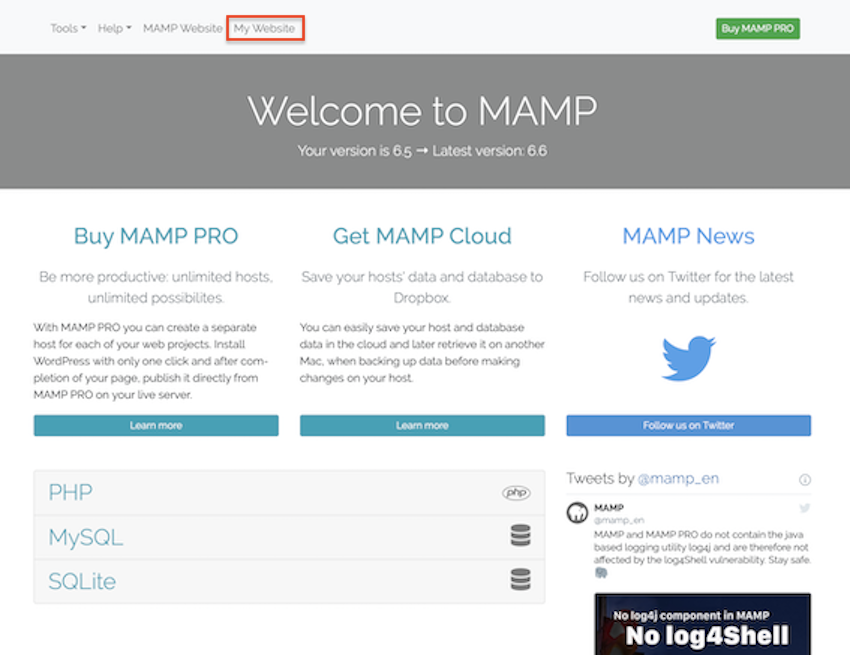
\includegraphics[width=10cm]{./img/MAMP_Web.png}
	\caption[MAMP interface]{The graphical interface provided by MAMP}
	\label{fig:MAMP_Web}
\end{figure}

\subsection{Drupal 9 installation}

Drupal 9 can be installed in two ways: by using drush, or by using the graphical user interface. 

Drush is, according to \textcite{Tomlinson2015}, \emph{"a command line tool that greatly simplifies the tasks of building and administering a Drupal website."} Drush allows you to perform specific tasks related to your Drupal website, one of which is installing the website.

For this proof of concept, the Drupal 9 graphical user interface will be used, as it is still the most straight forward way of installing Drupal. When using this interface, Drupal 9 will prompt you through a few steps:

\begin{enumerate}
	\item Choosing the default installation language.
	\begin{figure}[h]
		\centering
		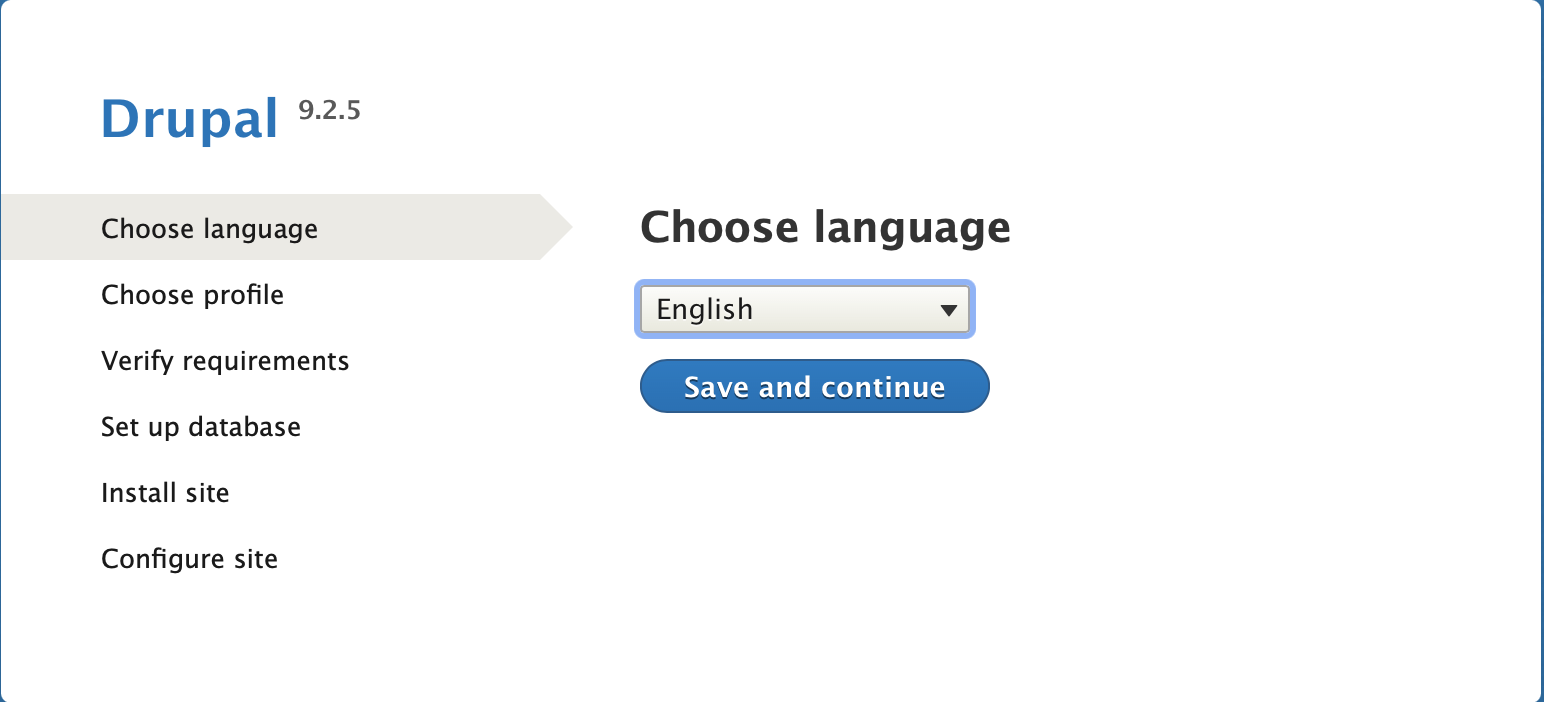
\includegraphics[width=10cm]{./img/Install_Language.png}
		\caption[Language choice]{Choosing a language in the Drupal 9 installation}
	\end{figure}
	\item Choosing an installation profile. Drupal 9 core comes with two default profiles that can be chosen. Firstly there is the standard profile. This profile comes with commonly used features already pre-configured. Secondly, the minimal profile is used to build a completely custom site without pre-configured functionality. There is also a demo profile included, which comes with some content already in the system. This can be used for testing out the possibilities of Drupal 9. For this research the standard profile will be used.
	\begin{figure}[h]
		\centering
		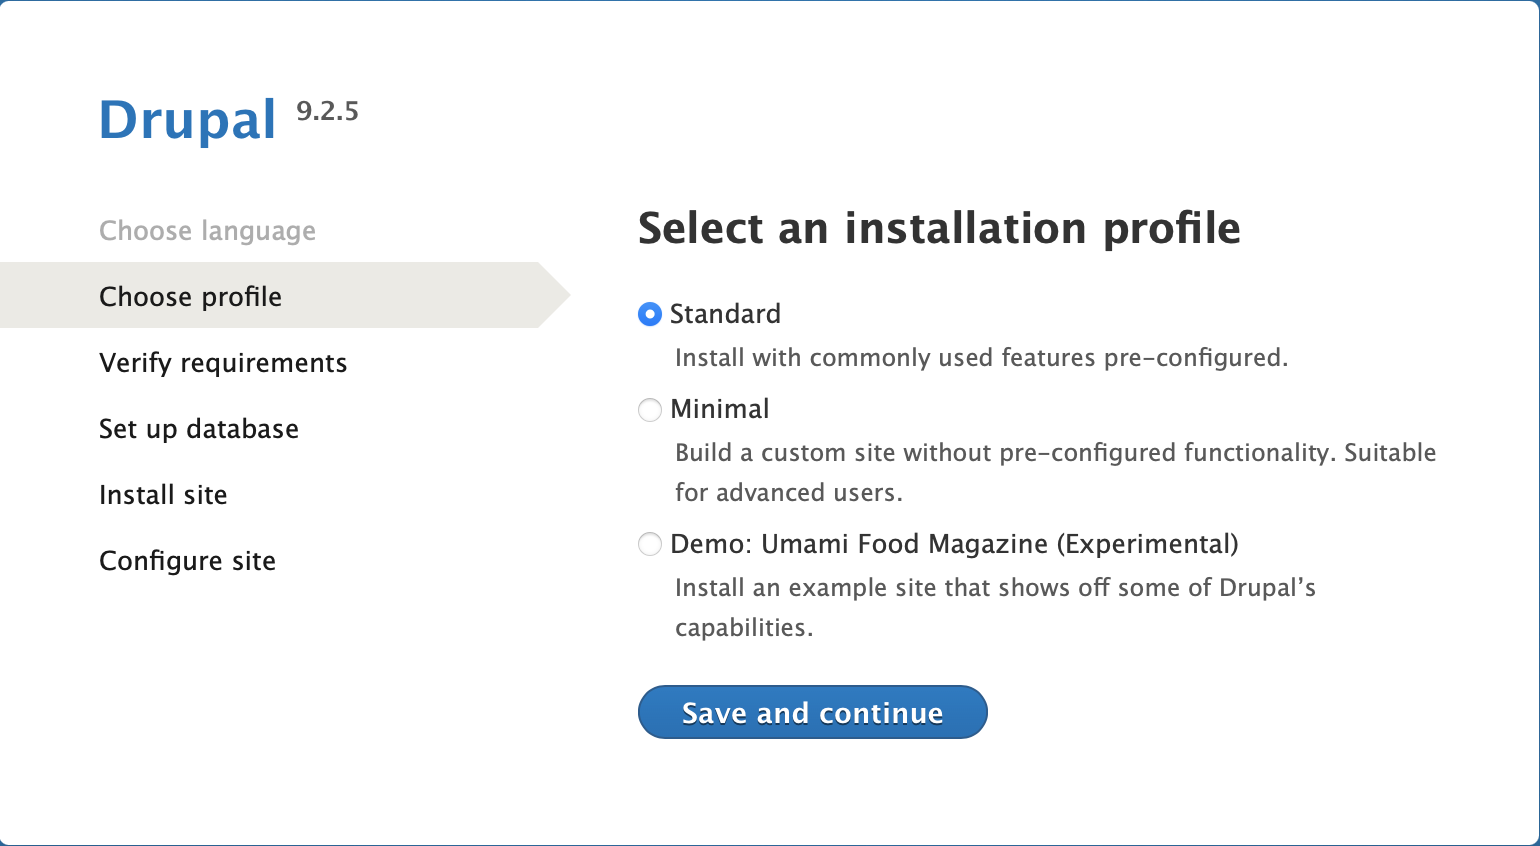
\includegraphics[width=10cm]{./img/Install_Profile.png}
		\caption[Install Profile Choice]{Choosing the install profile in the Drupal 9 installation}
	\end{figure}
	\item Setting up the database. In most cases, this step will be configured automatically by the installer. In some rare occasions though, there might be an issue that needs to be resolved by the site administrator.
	\item Install site. This step will automatically install the Drupal 9 site on your system. As with the previous step, there might be some issues that need to be resolved before the installation can be completed.
	\item Configuration of the site. In this step, you will be asked to configure some important settings. The site information, including the site name and e-mail address, need to be filled in, and you will need to configure an administration account for your website. The name of this account is usually \emph{admin}. After that, regional settings and update information need to be configured.
	\begin{figure}
		\centering
		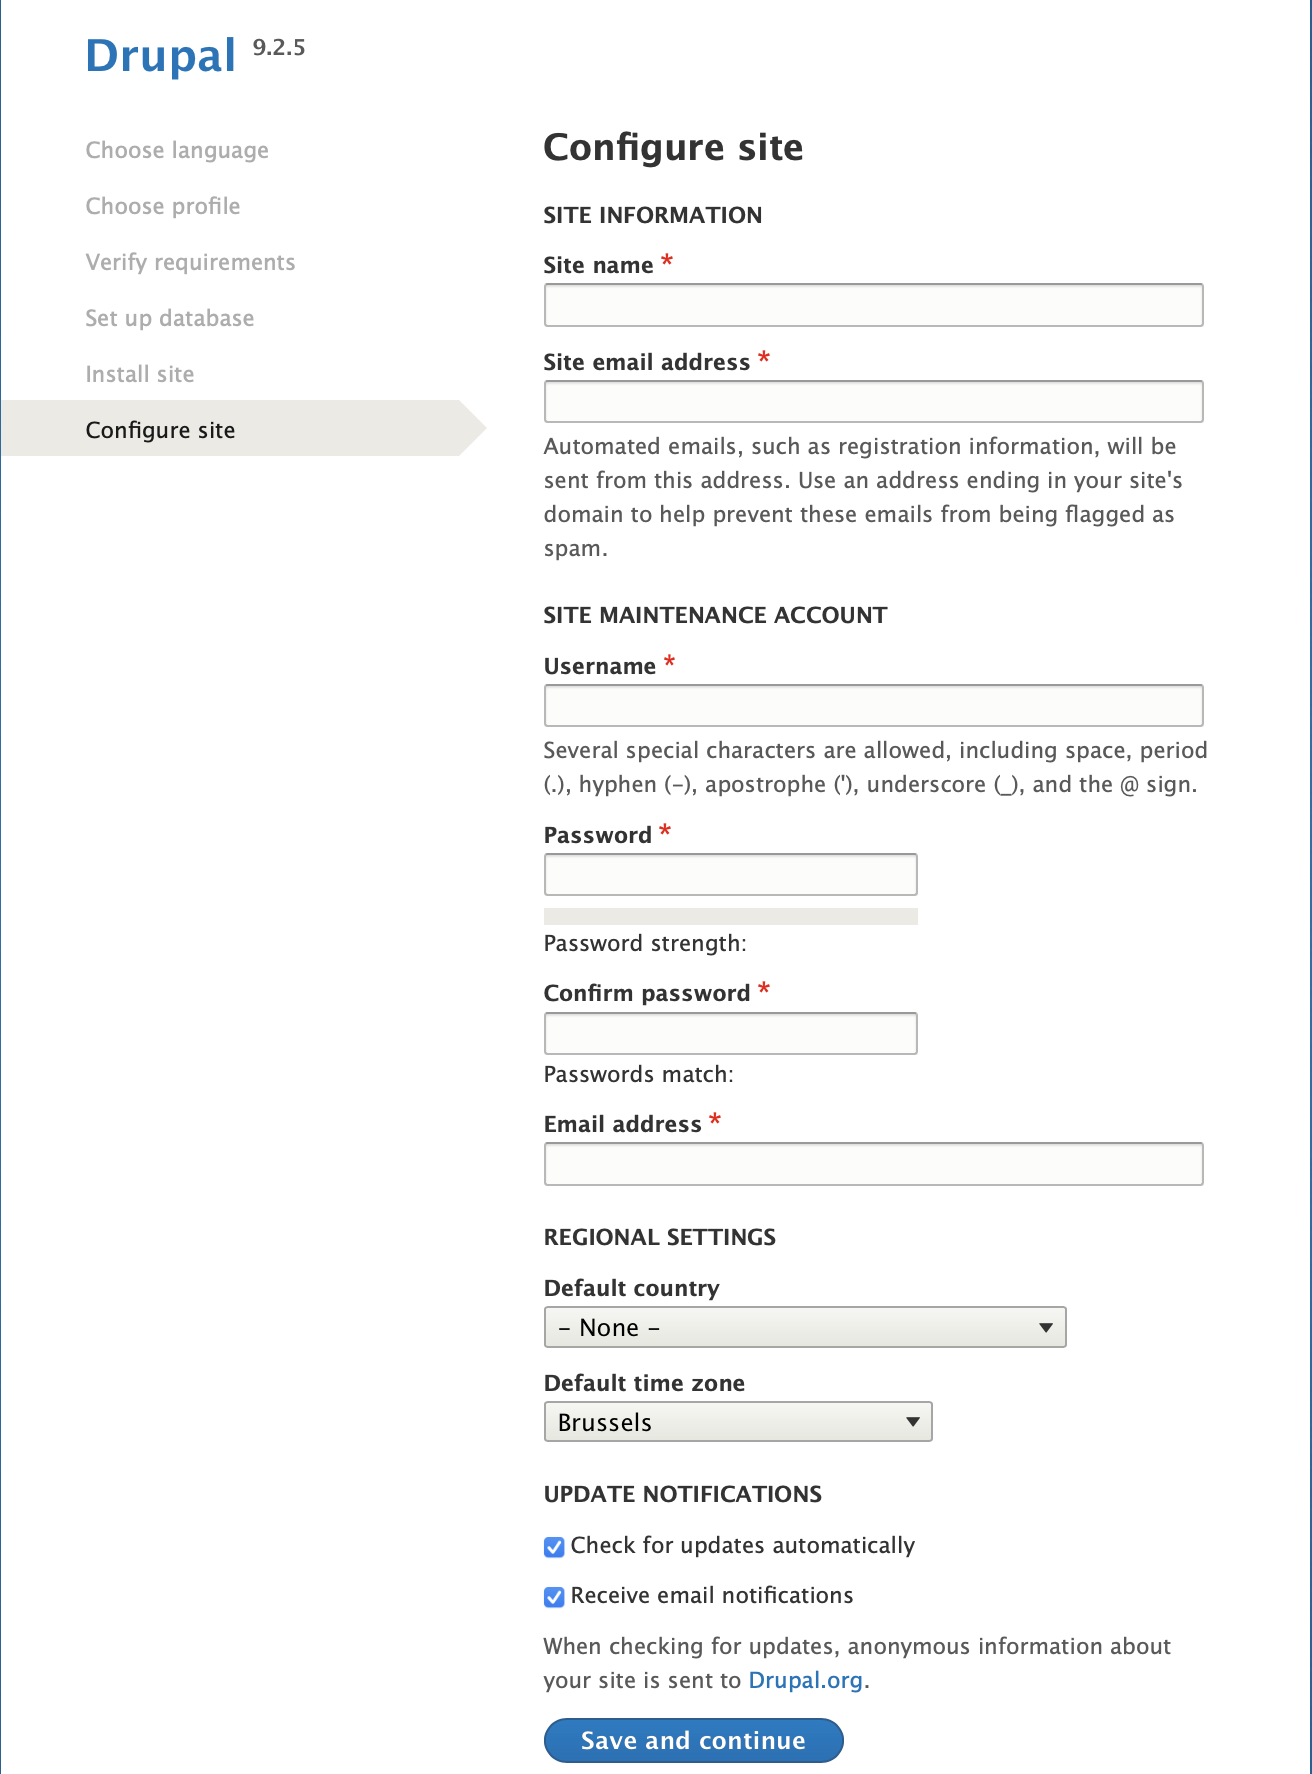
\includegraphics[width=10cm]{./img/Install_Config.png}
		\caption[Configuring Drupal 9]{Configuring your Drupal 9 site}
	\end{figure}
\end{enumerate}

When all these steps are completed, a new Drupal 9 site is ready for use. Before getting started with adding content to the site, there are a few optional things to do to improve the user experience.

\subsubsection{Installing modules and themes}

Installing modules in Drupal 9 is a fairly simple process. Modules that are included in Drupal 9 core can be easily enabeled through the user interface by going to \url{http://localhost:8888/admin/modules}. Contributed modules, available on \url{https://www.drupal.org} are a little trickier. The best way to install these is via the use of \emph{Composer}. According to \textcite{So2018} Composer is a dependency manager for PHP. It can be compared to NPM (Node Package Manager) for JavaScript. Using Composer, new modules can be easily installed by running the 'composer require' command in the root of your Drupal project. In the case of this proof of concept, the root directory is \emph{htdocs}. On other environments, the root directory is often called \emph{docroot}.

One module that can improve the user experience in Drupal is the \emph{Admin Toolbar}
module the most recent version can be installed by using Composer: "composer require 'drupal/admin\_toolbar:3.1'". This module improves the default toolbar by transforming it into a  drop-down. It also has three sub-modules that can be enabled for further customizing the admin toolbar.

In this proof of concept the Drupal front-end will not be used, so installing a theme for that would not do much. But installing an administration theme is something that could be a good idea. Themes can always be found on \url{https://www.drupal.org}. As an example, the \emph{Gin} administration theme can be installed by running "composer require 'drupal/gin:3.0@beta'". This theme can then be enabled by going into the appearance settings of the site, installing the theme and choosing it to be the administration theme. The theme is now applied, and it is now safe to uninstall any other themes that are not used. For this proof of concept, the \emph{Seven} theme will be used for administration purposes. This theme comes pre-installed with Drupal 9 core and has a very recognizable look and feel.

\subsection{Adding content}

Content is the core of any traditional CMS. For the purposes of this proof of concept, to show off the possibilities of headless, two different content types will be made that can later be exposed to front-end applications: a \emph{Book} content type and an \emph{Author} content type.

The \emph{Book} content type will have the following fields: 

\begin{itemize}
	\item Title
	\item Abstract
	\item Image (this field will not contain an actual image, but will contain a URL pointing to the image)
	\item Author (this field will be a reference field referencing the \emph{Author} content type)
\end{itemize}

The \emph{Author} content type will contain the following fields:

\begin{itemize}
	\item First Name
	\item Last Name
\end{itemize}

New content types can be created by going to \url{http://localhost:8888/admin/structure/types} and selecting the \emph{add new content type} option. This will allow you to configure any fields you want to be present on your content type.


\section{Exposing data}

At the basis of using a headless CMS lies the exposing of data. This means that the data that is available within the CMS is exposed through the use of a file format like JSON or XML, just like it would be done in a traditional web API. When correctly configured, any source can then ask for and receive that data, after which they can do with it as they like. Data can also be sent back to the CMS by client applications. In Drupal 9 there are two main modules that fulfill this purpose: JSON:API and RESTful Web Services.

\subsection{The JSON:API module}

The JSON:API module is included in Drupal 9 Core, so there is no need to install it using composer. The module can be enabled by going to \url{http://localhost:8888/admin/modules}. When installing this module, the \emph{Serialization} module will be automatically installed as well, as it is a dependency for JSON:API.

\begin{figure}[h]
	\centering
	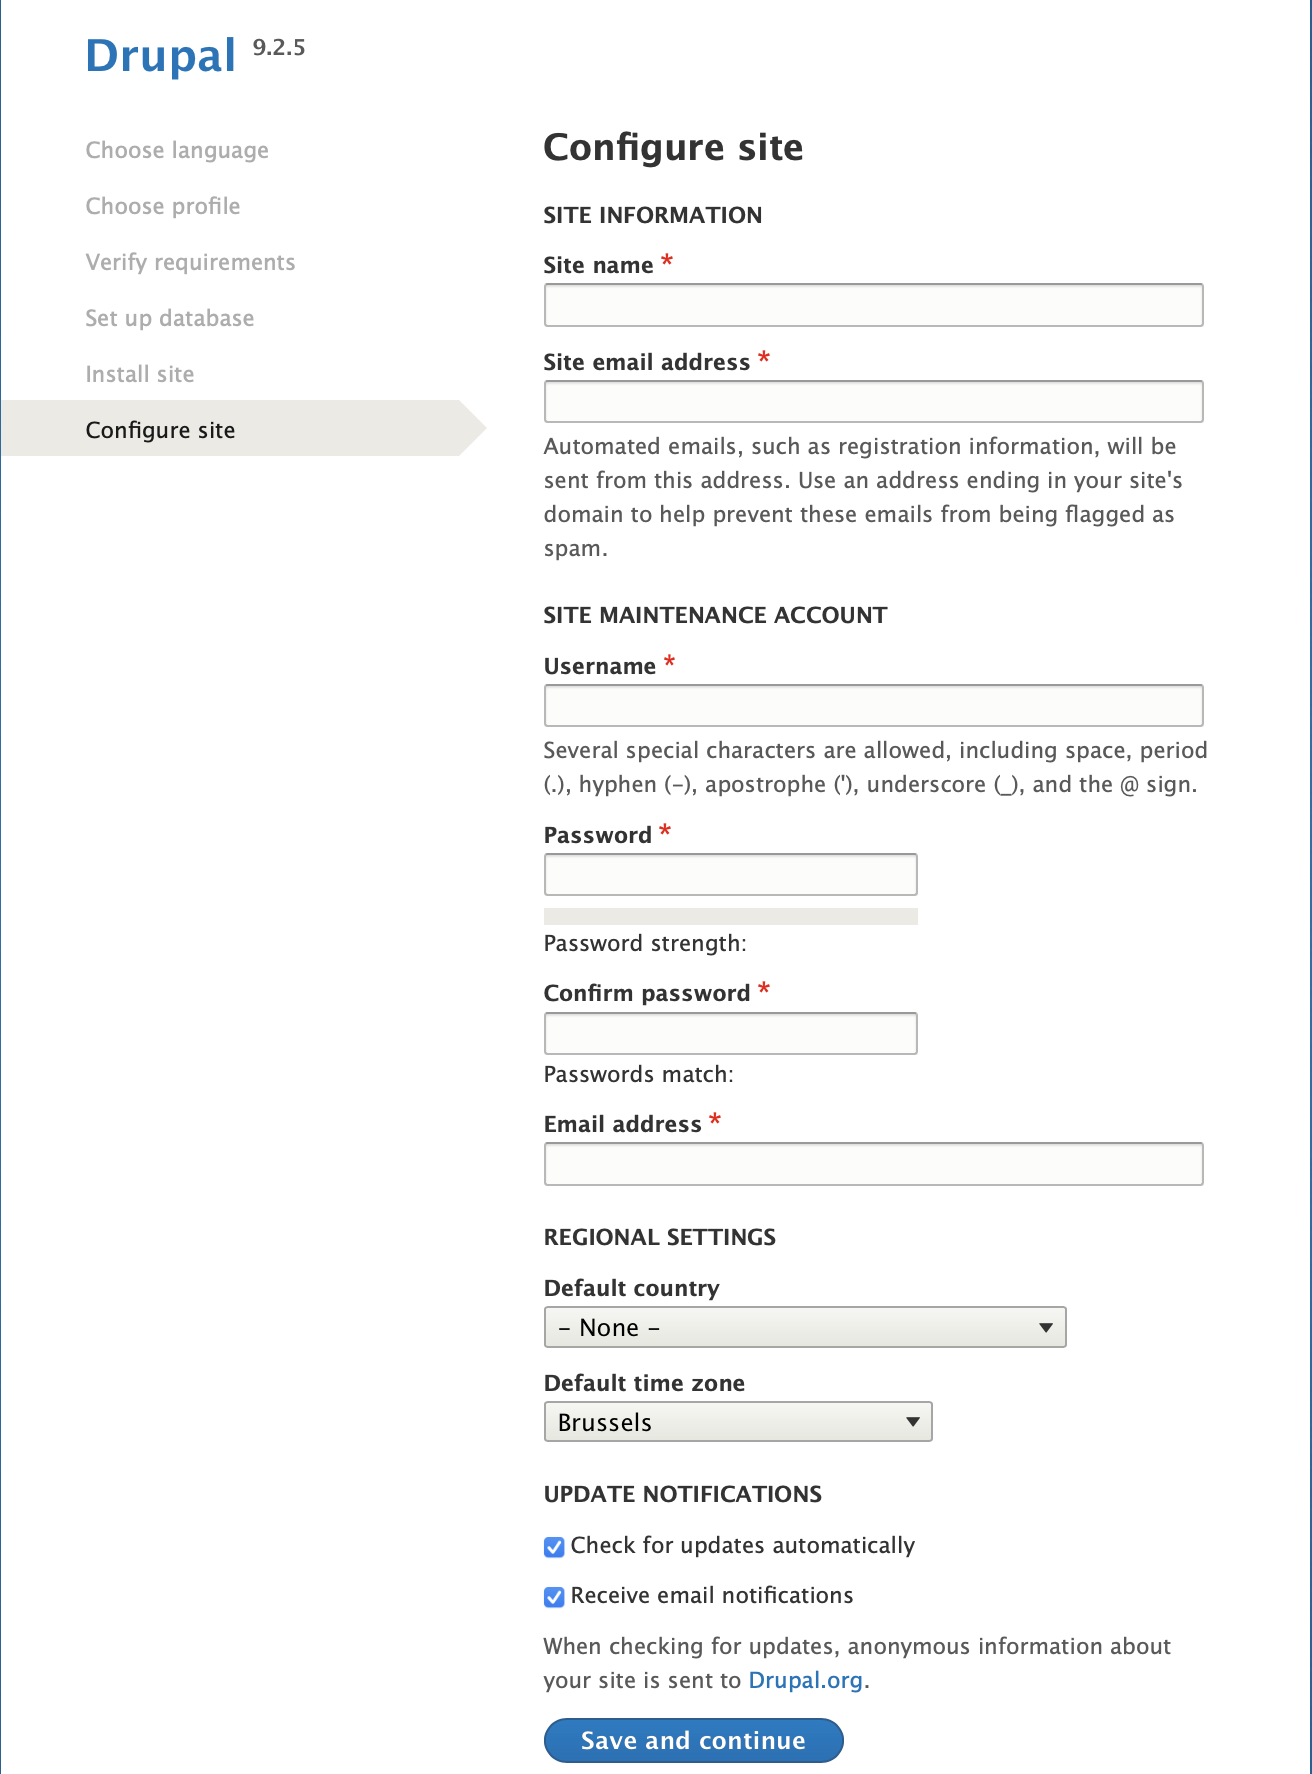
\includegraphics[width=10cm]{./img/Install_Config.png}
	\caption[Configuring Drupal 9]{Configuring your Drupal 9 site}
\end{figure}

As explained earlier in section \ref{sss:JSONAPI}, no configuration is needed to make this module work. The only piece of configuration that exists here is the choice to allow all operations (create, read, update and delete) instead of just read operations. By default only read operations are accepted. This configuration can be found by going to \url{http://localhost:8888/admin/config/services/jsonapi}. For this example this option will be turned on.

When this module is enabled, all of the content available in the system will be exposed in a standard, fixed format. This content, in JSON (JavaScript Object Notation) format, can be found at \url{http://localhost:8888/jsonapi/node/{content_type}} For our \emph{Book} content type (\url{http://localhost:8888/jsonapi/node/book}), this looks like this:

\begin{lstlisting}
{
	"jsonapi": {},
	"data": [
	{
		"type": "node--book",
		"id": "4b82e6d3-8138-484d-8c9e-5689ba65a671",
		"links": {},
		"attributes": {
			"drupal_internal__nid": 2,
			"drupal_internal__vid": 2,
			"langcode": "en",
			"revision_timestamp": "2022-05-22T11:42:24+00:00",
			"revision_log": null,
			"status": true,
			"title": "Harry Potter and the Philosopher's Stone",
			"created": "2022-05-22T11:37:07+00:00",
			"changed": "2022-05-22T11:42:24+00:00",
			"promote": true,
			"sticky": false,
			"default_langcode": true,
			"revision_translation_affected": true,
			"path": {},
			"field_abstract": {
				"value": "<p>Harry Potter and the Philosopher's Stone&nbsp;is a&nbsp;fantasy novel&nbsp;written by British author&nbsp;J. K. Rowling. The first novel in ...</p>"
			},
			"field_image": "https://upload.wikimedia.org/wikipedia/en/6/6b/Harry_Potter_and_the_Philosopher%27s_Stone_Book_Cover.jpg"
		},
		"relationships": {
			"node_type": {},
			"revision_uid": {},
			"uid": {},
			"field_author": {
				"data": {
					"type": "node--author",
					"id": "24efb772-0b6f-4ad8-942f-05cf4e725ba9"
				},
				"links": {}
			}
		}
	}
	],
	"links": {}
}
\end{lstlisting}

This is what is called an \emph{end point}. The url of this end point can be used by other applications to get the data that is displayed here. The most important parts of this data are:

\begin{itemize}
	\item \emph{data}: contains all the pieces of content of that specific content type. In this case, this is a list of books.
	\item \emph{type}: shows the content type of this piece of content
	\item \emph{id}: the id of this piece of content.
	\item \emph{attributes}: contains all the data of this piece of content. In this case, for example, it contains the title, abstract and image fields of the book.
	\item \emph{relationships}: contains the id of any reference fields that might be present on this piece of content. In this case, the id of the author that wrote this book is shown.
\end{itemize}

For the authors, a similar end point can be found at \url{http://localhost:8888/jsonapi/node/author}. With any content types there is also the possibility to look up just a single piece of content, instead of showing the entire list. This can be very useful if your site contains a lot of content of a specific type, because having to pull all of these in at once can consume time and resources. Getting a single piece of content can be achieved when the id of the content is known. For example, a single book can be found at \url{http://localhost:8888/jsonapi/node/book/{id}}, with \{id\} being replaced by the id of a specific book.

As you can clearly see, using this module is a very easy way to expose the data of any content types in your system. This is the big upside to using this method. The downside is that you do not have a lot of control over what data gets exposed. It will always be all content types, and will always have a set structure that cannot be changed.


\subsection{The  RESTful Web Services module}



\section{The front-end}

There are many options to consider on the front-end. These range from javascript frameworks to native mobile applications. Basically any framework or tool that has a way to handle HTTP request throught the use of an HTTP client has the possibility to interact with a headless CMS. For this research, the choice was made to use the front-end javascript framework Angular. Angular is an extremely popular framework used around the world to create single page applications. It also has a built-in HTTP client that can be used to create any HTTP request and send it to any domain.

\subsection{Single page web application with Angular}

\subsection{Mobile application with SwiftUi}